%experiment
Das SLM-Toolkit ist ein Werkzeug von Roni Rosenfeld, das angegebene Texte bearbeitet und folgende Ausgaben erzeugt\cite{int_slm_toolkit}:
\begin{itemize}
	\item H\"aufigkeitsliste der Worte und Vokabular
	\item H\"aufigkeit von Bigramen und Trigrammen
	\item Statistik des Bigramms und Trigramms
	\item Bigramm-und Trigramm-Modell mit unterscheidlichen Backingoff-Methoden
	\item Perplexit\"at
	\item Bigramm- und Trigramm-Hit-Auftrittsrate der Testkorpora
	\item Verteilung unter Backingoff-Methode 
\end{itemize}
Die Software gibt beim Sprachmodell auch "`absolute"', "`good\_turing"' and "`witten\_bell- Discounting"' an.
F\"ur ein bestimmtes Ziel muss man nicht alle Software ausf\"uhren. Abbildung (3.1) zeigt eine typische Anwendung, die Datenfluss und Operationfluss darstellt.
Ein Trainingskorpus wird zu Beginn eingegeben und nach dem Modellierungsverfahren wird ein Sprachmodell ausgegeben
\begin{figure}[h]
	%\centering
	\centering
	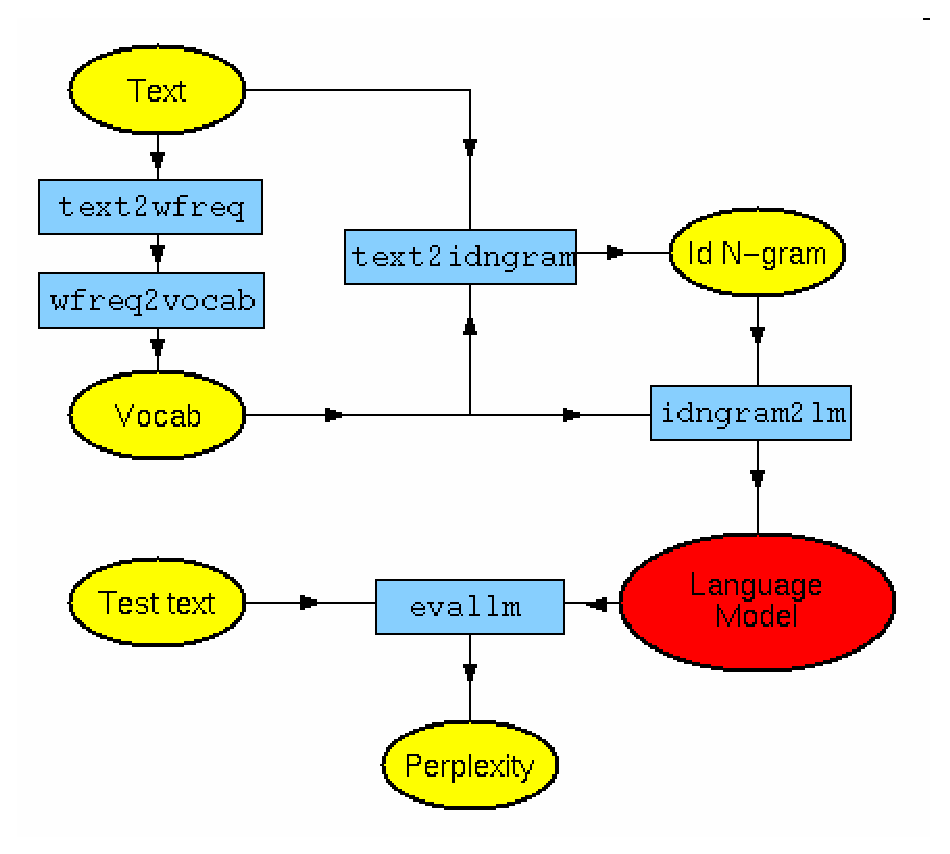
\includegraphics[width=0.5\textwidth]{bilder/toolkit.eps}
	 \caption{Flussdiagramm der typische Anwendung}
  \label{fig:figure_2}
\end{figure}
Der Trainingskorpus und der Testkorpus m\"ussen sorgf\"altig entworfen werden. \cite{book_speech} deutet uns einige Regeln an, dass Trainingskorpora nicht zu spezifisch f\"ur die Aufgabe und auch nicht zu allgemein sein sollen.  
\\
\\
In unseren Experimenten verwenden wir die WSJ (Wall Street Journal) Sprachdatenbank und wir erhalten die Testergebnisse von unterschiedlichen Discounting und M-Gramm-Modellen. In den Experimenten werden am Ende die Parameter \emph{backoff\_from\_un-k\_inc} und \emph{backoff\_from\_unk\_exc} beim Entropieberechnen eingesetzt. Der Unterschied zwischen beiden Parametern wird in \cite{int_slm_toolkit} erkl\"art, dass in dem Fall des Null-Wahrscheinlich-keit-Problems nur die Wahrscheinlichkeit vom (M-1)-Gramm unter dem Parameter \emph{backoff\_from\_unk\_inc} und auch die Wahrscheinlichkeit vom (M-2)-Gramm unter dem Parameter \emph{backoff\_from\_unk\_exc} verwendet werden.
\\
\\  
Aber es wurde auch eine Problem gefunden, dass beim Absolute-Discounting man nur NAN bekommen kann, wenn man mit komplette wsj-Databasis arbeitet, weil die Vokabulargr\"o\ss e auf 65535 beschr\"anket wird. In der Tabelle 3.1 wird nur die verringerte Trainingbasis (Trainingdaten aus Verzeichnis 88 und Testdaten "`pp\_et\_05.nvp"') angegeben. Die Testdatei "`pp\_et\_05.nvp"' ist von der Trainingbasis unabh"angig.
%table
%table 3.1
\begin{table}[h]
  \begin{center}
  \small\addtolength{\tabcolsep}{-5pt}
    \begin{tabular}{l|l|r|r|r|r|r|r}
     \toprule
     m- &Backoff &\multicolumn{2}{|l|}{Absolute}&\multicolumn{2}{|l|}{Witten-bell}&\multicolumn{2}{l}{Good-Turing}\\
	  \cline{3-8}
	  Gram&(inc/exc)&Perplexit\"at&Entropie&Perplexit\"at&Entropie&Perplexit\"at&Entropie\\
    \hline
    \hline
		Trigramm &inc 	& $292.23$ 	& $8.19$ 	& $291.88$ 	& $8.19$ 	& $307.33$ 	& $8.26$\\
				 		 &exc		& $265.46$ 	& $8.05$ 	& $265.32$ 	& $8.05$ 	& $273.97$ 	& $8.1$\\
		\hline
		Bigramm  &inc 	& $354.2$ 	& $8.47$ 	& $353.4$ 	& $8.47$ 	& $359.32$ 	& $8.49$\\
				 		 &exc		& $330.24$ 	& $8.37$ 	& $329.74$ 	& $8.37$ 	& $334.73$ 	& $8.39$\\
		\hline
		Unigramm &inc 	& $1130.39$ & $10.14$ & $1130.39$ & $10.14$ & $1130.39$ & $10.14$\\
				 		 &exc		& $1130.39$ & $10.14$ & $1130.39$ & $10.14$ & $1130.39$ & $10.14$\\
     \bottomrule
    \end{tabular}
  \end{center}
     \caption{Die Entropie und Perplexit\"at aller Discountings und unterschiedlichen M-Gramme}
\label{tab:table_3}
\end{table}
\\
\\
Aus obigen Testergebnissen kann man als Fazit festhalten, dass Trigramme besser als Bigramme sowie Unigramme sind, \emph{backoff\_from\_unk\_exc} auch besser als \emph{backoff\_from\_u-nk\_inc} . 